%===============================================================================
% Planteamiento del problema.
% Autor(es): Landa
%	     David 
% 	     Alan
% Fecha: 12 - Mar - 2018
%
%===============================================================================

\section{Drones}

%% Descripción general
%
\subsection{Concepto de drone}

Los drones o vehículos aéreos son casi todo lo que está en el aire sin un 
piloto, un globo con un termómetro, un multicopter con una cámara integrada y 
posiblemente un avión militar portador de misiles. Este tipo de vehículos pueden 
adoptar diversas formas, ya que, dependiendo del modelo, pueden ser dirigidos 
por un control remoto, así como volar de forma autónoma siguiendo su GPS (Global 
Position System) \cite{drone_nombre_cosa}. \\
Técnicamente, a los drones se les suele denominar VANT (Vehículo Aéreo No 
Tripulado) o por sus siglas en inglés UAV (Unamed Aereal Vehicles), finalmente 
son aeronaves no tripuladas por algún piloto 
\cite{app_veh_no_tripulados_hidr, drone_nombre_cosa}. \\
Es un aparato que vuela sin que nadie a bordo lo tripule y dirija. Sigue 
instrucciones de una base desde tierra. \\
Uno de los problemas a los que se enfrentan esta clase de aparatos aéreos frente 
al público en general, es que ningún organismo oficial, indiferentemente al 
país, ha regulado y definido con propiedad cómo conceptualizar a cada tipo de 
aparato \cite{drone_nombre_cosa}.

%% Características de un drone. 
%
\subsection{Características de un drone}

Los drones comúnmente pueden variar de acuerdo con su tamaño, ya que podemos 
encontrar drones del tamaño mini, hasta del tamaño de aviones de carga 
\cite{fisica_quadcoptero}. \\
En el caso de drones civiles, los drones no presentan gran tamaño, al contrario, 
son ligeros, desmontables, e inclusive pueden llegar a transportarse en una 
maletera. \\
Para poder entender el mundo de los drones, necesitamos saber cómo está 
estructurado, es decir, los componentes que tiene en su infraestructura que le 
permiten mantener un vuelo estable \cite{fisica_quadcoptero}:

\begin{itemize}
	\item \textbf{Chasis o frame}. 
		Compuesto por fibra de carbono, para facilitar ligereza y 
		resistencia.
	\item \textbf{Controladora de vuelo o de autopiloto}. 
		Con el objetivo de mantener el estado de vuelo, esta puede 
		disponer de dispositivos como GPS, giroscopio, barómetro, 
		magnetómetro, WiFi, cámara. etc.
	\item \textbf{Motores}. 
		Estos dispositivos, son los encargados de suministrar la energía 
		necesaria a las hélices para sustentar la aeronave.
	\item \textbf{Hélices}. 
		 Se caracterizan principalmente por el número de palas, el paso, 
		dirección de giro, tamaño, el material de las cuales están 
		compuestas.
	\item \textbf{Control de velocidad eléctrico (ESC)}. 
		Se clasifican de acuerdo con la cantidad de corriente que 
		suministran a los motores.
	\item \textbf{Placa distribuidora de energía}. 
		Esta placa está formada por la conexión que va de los ESC al 
		punto de conexión de la batería.
	\item \textbf{Baterías}. 
		Son baterías de tipo Li-Po (Litio-Polímero), ya que dependiendo 
		del drone pueden tener por lo menos tres celdas, de al menos 
		3.7V cada una, y con capacidad regulable según ciertos factores.
	\item \textbf{Emisor-Receptor}. 
		 Los drones normalmente tienen internamente un dispositivo 
		receptor y emisor que permiten comunicarse con un control 
		remoto.
\end{itemize}

Los drones comerciales, ofrecen una batería, la cual puede llegar a durar entre 
los 30 minutos, o 60 minutos, dependiendo de la robustez del aparato. \\

Estos dispositivos cuentan con un gran potencial, ya que, pueden desplazarse en 
zonas de alto riesgo o de difícil acceso, superar obstáculos, pueden ofrecer 
imágenes aéreas, fáciles de controlar, sin necesidad de poner en peligro la vida 
de civiles.  

%% Clasificación de drones
%
\subsection{Clasificación de drones}
De acuerdo con los desarrollos de vehículos aéreos no tripulados se encuentra 
una clasificación con base en su diseño 
\cite{app_veh_no_tripulados_hidr, x_drone_clasificacion}:

\begin{enumerate}
	\item UAV de ala fija. \\
	Se refiere a aeroplanos con alas, los cuáles requieren de una pista para 
	despegue y aterrizaje. Tiene bastante autonomía de vuelo y, además, 
	pueden volar a altas velocidades. \\
	A su vez este tipo de drones se pueden clasificar por sus 
	características físicas, como:  \\
	Por medio de balance levantamiento/masa, por su estabilidad, Por su 
	control:

	\begin{itemize}
		\item Estabilizador en popa (Tailplane aft).
		\item Estabilizador hacia adelante (Tailplane forward).
		\item Sin cola (Tailess).
	\end{itemize}

	\item UAV de ala rotatoria. \\
	Son UAVs de despegue y aterrizaje vertical, los cuales poseen ventajas 
	en su capacidad de permanecer en el aire y brindar una alta 
	manejabilidad. \\
	Algunos nombres que se conoce a los drones de este tipo son:

	\begin{itemize}
		\item De un solo rotor. \\
		Básicamente es un helicóptero de un solo rotor arriba, y debe 
		contrarrestarse con otro rotor en la cola para evitar torque por 
		el rotor principal.
		\item De rotor coaxial. \\
		Posee dos rotores simétricos en el mismo eje. Es de fácil 
		manipulación.
		\item De rotor en tándem o multirotor. \\
		Estos son de diversos tipos, ya que en función del número de 
		rotores independientes que poseen. De estos, destacan los 
		cuadricópteros, hexacópteros, se pueden encontrar una gran 
		variedad de modelos en el mercado.  
	\end{itemize}

\end{enumerate}

%% Fabricantes
%
\subsection{Fabricantes de drones}

\begin{figure}[H]
	\begin{center} 
		\includegraphics[scale=0.4]{images/doc/img_fabricantes_drones}
		\caption{Fabricantes de drones en el mundo.}
	\end{center}
\end{figure}

Diversas compañías a lo largo del mundo han estado compitiendo por el mercado de
los drones, entre ellas han aportado diversos diseños propios de cada una, 
además, agregado diversos componentes, estructuras de fuselaje, baterías, 
potencia de motores, sistemas operativos embebidos, calidad de calibración del 
GPS, giroscopio, entre otros componentes que han proporcionado un gran número de 
aplicaciones que han realizado diversos usuarios en todo el mundo 
\cite{x_drone_clasificacion}. \\

Los fabricantes mas dominantes se muestran en la figura \ref{grafica:fabricantes}, con un ranking de 2016-2017 \cite{drone_industry_insights, companias_dominantes_drones}.

\begin{figure}[H]
	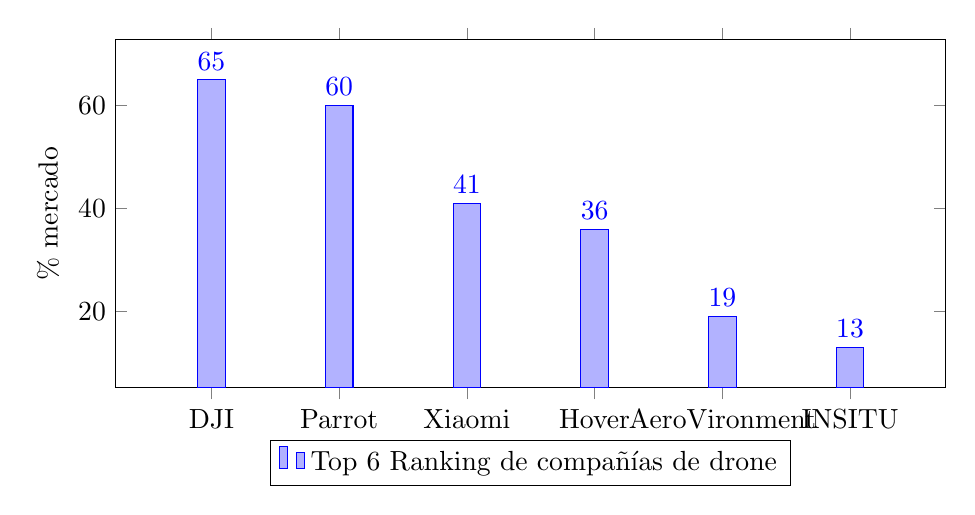
\begin{tikzpicture}	
	\begin{axis}[
	ybar,
	enlargelimits=0.15,
	legend style={at={(0.5,-0.15)},
		anchor=north,legend columns=-1},
	ylabel={\% mercado},
	symbolic x coords={DJI,Parrot,Xiaomi,Hover,AeroVironment,INSITU},
	xtick=data,
	nodes near coords,
	nodes near coords align={vertical},
	width=1.0\textwidth,
	height=6cm,
	]
	\addplot coordinates {(DJI,65) (Parrot,60) 
		(Xiaomi,41) (Hover,36)
		(AeroVironment,19) (INSITU,13)};
	\legend{Top 6 Ranking de compañías de drone}
	
	\end{axis}
	\end{tikzpicture}
	
	\caption{Ranking de compañías que dominan el mercado de fábrica de drones.}
	\label{grafica:fabricantes}
\end{figure}
